The following sections describe the set of demos that have been compiled to
demonstrate some of the features and usage of the risk calculators of the
\glsdesc{acr:oqe}. These demos can be found in a public repository on GitHub at
the following link:
\href{https://github.com/gem/oq-engine/tree/master/demos/risk}
{https://github.com/gem/oq-engine/tree/master/demos/risk}.

These examples are purely demonstrative and are not intended to represent
accurately the seismicity, vulnerability or exposure characteristics of the
region selected, but simply to provide example input files that can be used
as a starting point for users planning to employ the \glsdesc{acr:oqe} in seismic
risk and loss estimation studies.

It is also noted that in the demonstrative examples presented in this section,
illustrations about the various messages from the engine displayed in the
command line interface are presented. These messages often contain information
about the calculation id and output id, which will certainly be different for
each user.

Following is the list of demos which illustrate how to use the \gls{acr:oqe} for
various scenario-based and probabilistic seismic damage and risk analyses:

\begin{itemize}

    \item ClassicalBCR
	\item ClassicalDamage
    \item ClassicalRisk
    \item EventBasedDamage
    \item EventBasedRisk
    \item ScenarioDamage
    \item ScenarioRisk

\end{itemize}

These seven demos use Nepal as the region of interest. An example
\gls{exposuremodel} has been developed for this region, comprising 9,063
assets distributed amongst 2,221 locations (due to the existence of more than
one \gls{asset} at the same location). A map with the distribution of the
number of buildings throughout Nepal is presented in Figure~\ref{fig:exposure-nepal}.

\begin{figure}[ht]
\centering
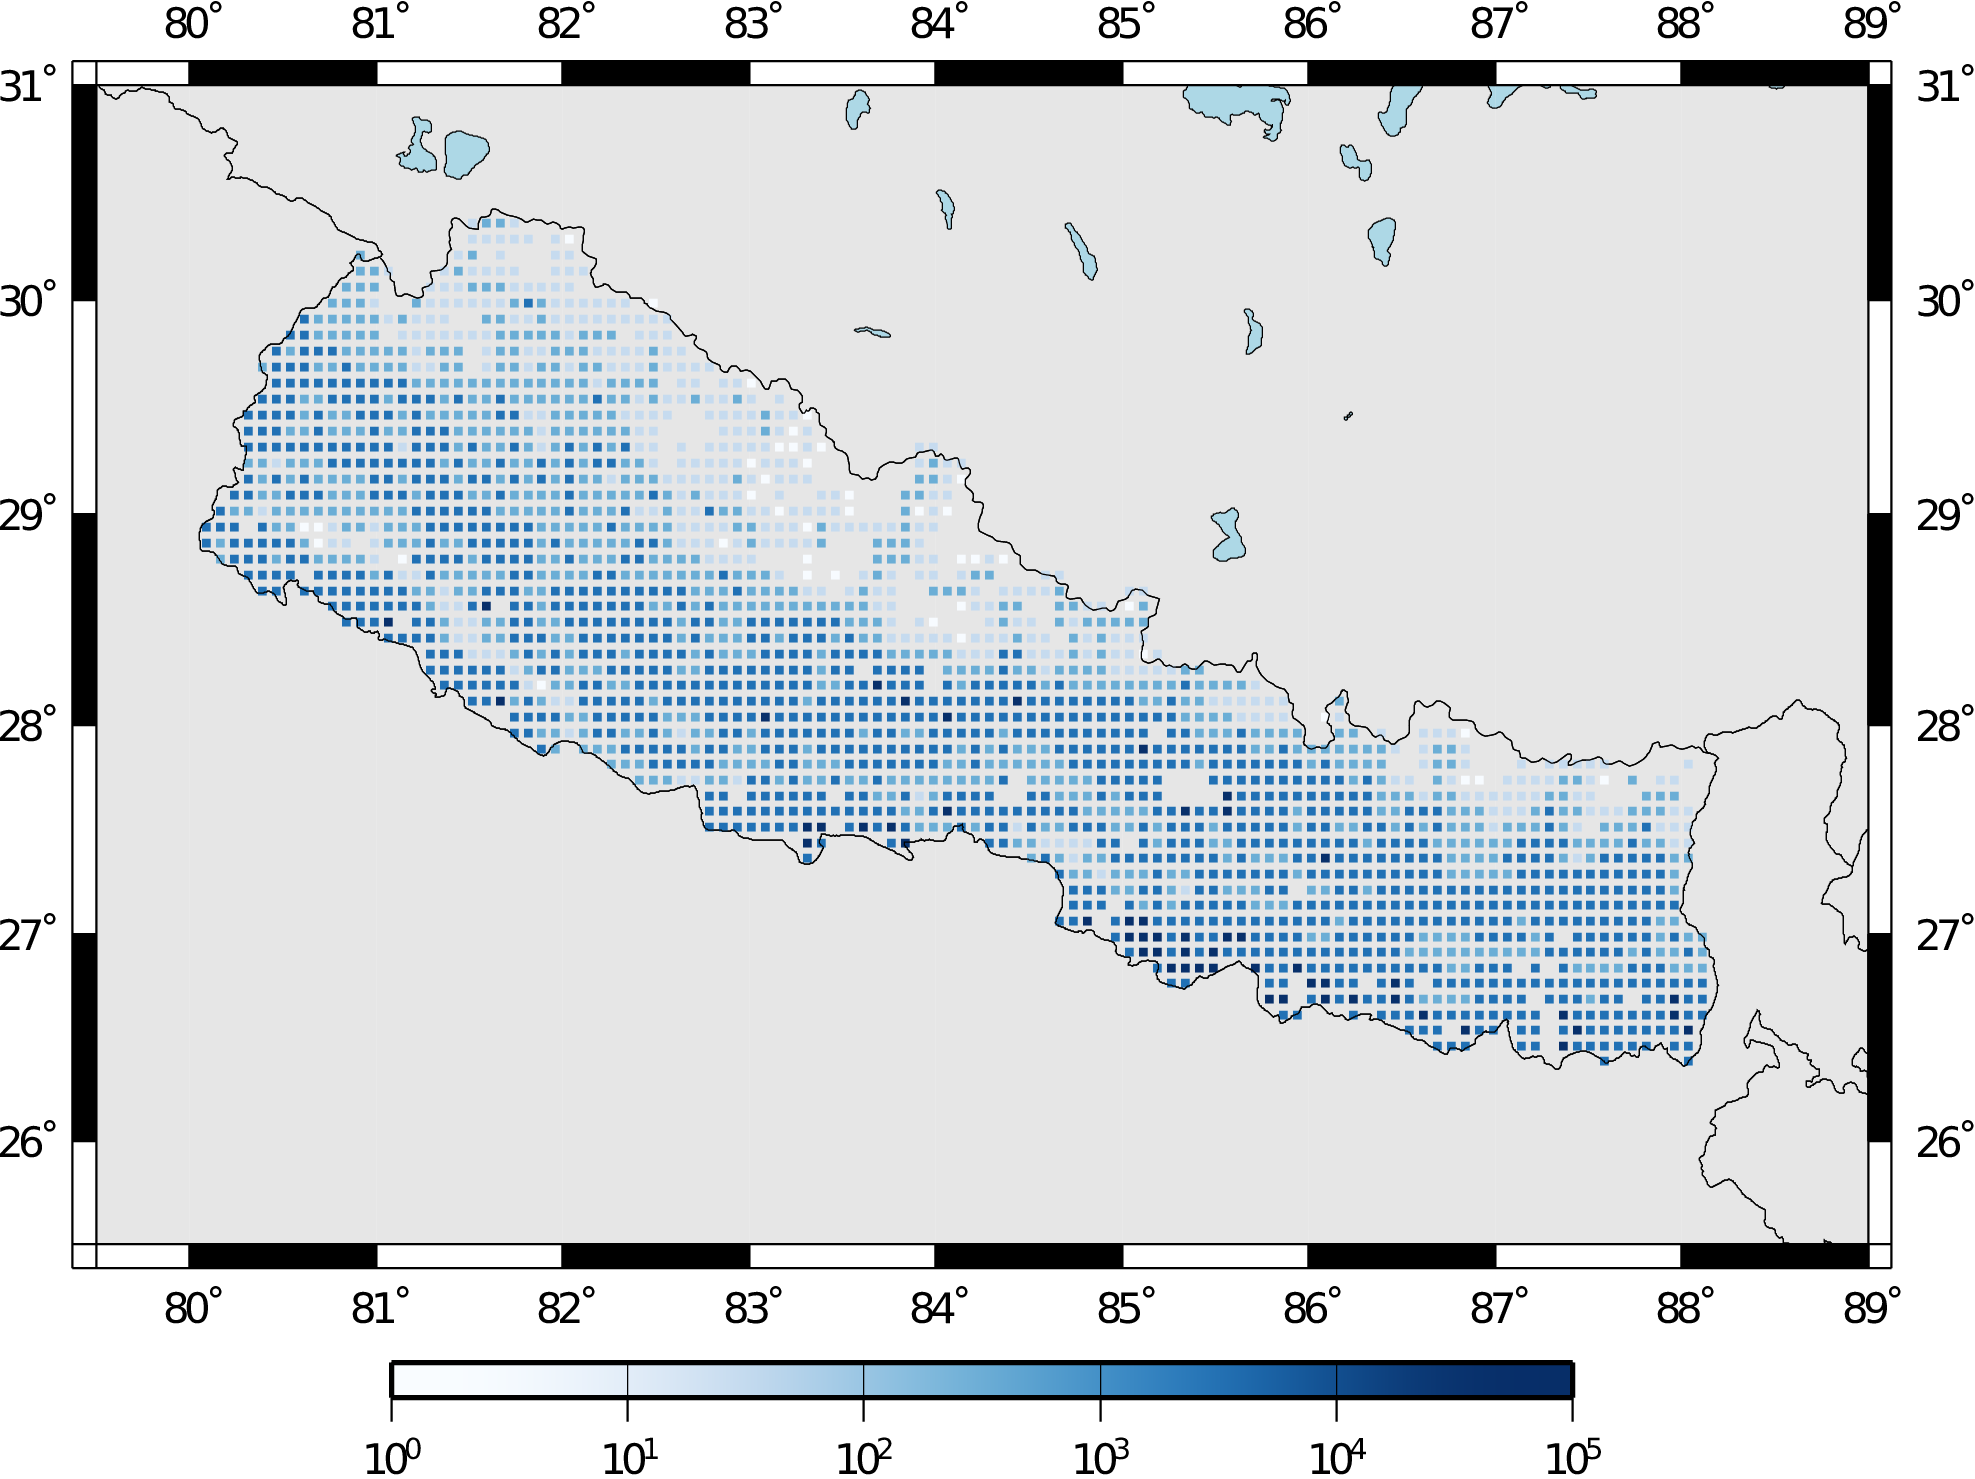
\includegraphics[width=12cm,height=8cm]{figures/risk/exposure-nepal.pdf}
\caption{Distribution of number of buildings in Nepal}
\label{fig:exposure-nepal}
\end{figure}

The building portfolio was organised into four classes for the rural areas
(adobe, dressed stone, unreinforced fired brick, wooden frames), and five
classes for the urban areas (the aforementioned typologies, in addition to
reinforced concrete buildings). For each one of these building typologies,
\glspl{vulnerabilityfunction} and \glspl{fragilityfunction} were collected
from the published literature available for the region. These input models are
only for demonstrative purposes and for further information about the building
characteristics of Nepal, users are advised to contact the National Society
for Earthquake Technology of Nepal (NSET -
\href{http://www.nset.org.np/}{http:www.nset.org.np/}).

The following sections include instructions not only on how to run the risk
calculations, but also on how to produce the necessary hazard inputs. Thus,
each demo comprises the configuration file, \gls{exposuremodel} and fragility or
vulnerability models fundamental for the risk calculations. Each demo folder
also a configuration file and the input models to produce the relevant hazard
inputs.


\section{Scenario Damage Demos}
\label{sec:demos_scenario_damage}
\input{oqum/risk/04_demos_scenario_damage}

\section{Scenario Risk Demos}
\label{sec:demos_scenario_risk}
\input{oqum/risk/04_demos_scenario_risk}

\section{Classical Probabilistic Seismic Damage Demos}
\label{sec:demos_classical_damage}
\input{oqum/risk/04_demos_classical_damage}

\section{Classical Probabilistic Seismic Risk Demos}
\label{sec:demos_classical_risk}
\input{oqum/risk/04_demos_classical_risk}

\section{Event Based Probabilistic Seismic Damage Demos}
\label{sec:demos_event_based_damage}
This demo uses the same probabilistic seismic hazard assessment (PSHA) model
described in the previous examples in Section~\ref{sec:demos_classical_damage}
and Section~\ref{sec:demos_classical_risk}. However, instead of hazard curves,
sets of ground motion fields will be generated by the hazard calculation of
this demo. Again, since there is only one branch in the logic tree, only one
set of ground motion fields will be used in the risk calculations. The hazard
and risk jobs are defined in a single configuration file for this demo. To
trigger the hazard and risk calculations the following command needs to be
used:

\begin{minted}[fontsize=\footnotesize,frame=single,bgcolor=lightgray]{shell-session}
user@ubuntu:~\$ oq engine --run job.ini
\end{minted}

and the following results are expected:

\begin{minted}[fontsize=\footnotesize,frame=single,bgcolor=lightgray]{shell-session}
Calculation 2 completed in 29 seconds. Results:
  id | name
  24 | Aggregate Event Damages
  30 | Aggregate Event Losses
  20 | Average Asset Damages
  21 | Average Asset Damages Statistics
  22 | Average Asset Losses
  23 | Average Asset Losses Statistics
  32 | Earthquake Ruptures
  25 | Events
  26 | Full Report
  27 | Ground Motion Fields
  28 | Hazard Curves
  29 | Input Files
  31 | Realizations
\end{minted}


\section{Event Based Probabilistic Seismic Risk Demos}
\label{sec:demos_event_based_risk}
This demo uses the same probabilistic seismic hazard assessment (PSHA) model
described in the previous examples in Section~\ref{sec:demos_classical_damage}
and Section~\ref{sec:demos_classical_risk}. However, instead of hazard curves,
sets of ground motion fields will be generated by the hazard calculation of
this demo. Again, since there is only one branch in the logic tree, only one
set of ground motion fields will be used in the risk calculations. The hazard
and risk jobs are defined in a single configuration file for this demo. To
trigger the hazard and risk calculations the following command needs to be
used:

\begin{minted}[fontsize=\footnotesize,frame=single,bgcolor=lightgray]{shell-session}
user@ubuntu:~\$ oq engine --run job.ini
\end{minted}

and the following results are expected:

\begin{minted}[fontsize=\footnotesize,frame=single,bgcolor=lightgray]{shell-session}
Calculation 8974 completed in 229 seconds. Results:
  id | name
1820 | Total Loss Curves
1821 | Total Loss Curves Statistics
1822 | Aggregate Loss Table
1823 | Average Asset Losses
1824 | Average Asset Loss Statistics
1826 | Asset Loss Maps
1827 | Asset Loss Maps Statistics
1828 | Average Asset Losses
1829 | Average Asset Losses Statistics
1830 | Earthquake Ruptures
1831 | Events
1832 | Realizations
\end{minted}

The number and the name of the outputs can change between
different versions of the engine.


\section{Retrofit Benefit-Cost Ratio Demos}
\label{sec:demos_benefit_cost}
\input{oqum/risk/04_demos_benefit_cost}